\documentclass[10pt,mathserif,aspectratio=169]{beamer}

\usepackage{graphicx,amsmath,amssymb,tikz,psfrag,booktabs,natbib,adjustbox}

\input {newcommand.tex}

%% formatting

\mode<presentation>
{
  \usetheme{default}
}
\setbeamertemplate{navigation symbols}{}
\usecolortheme[rgb={0.13,0.28,0.59}]{structure}
\setbeamertemplate{itemize subitem}{--}
\setbeamertemplate{frametitle} {
  \begin{center}
    {\large\bf \insertframetitle}
  \end{center}
}

\newcommand\footlineon{
  \setbeamertemplate{footline} {
    \begin{beamercolorbox}[ht=2.5ex,dp=1.125ex,leftskip=.8cm,rightskip=.6cm]{structure}
      \footnotesize \insertsection
      \hfill
      {\insertframenumber}
    \end{beamercolorbox}
    \vskip 0.45cm
  }
}
\footlineon

% backup slides
\usepackage{appendixnumberbeamer}
\newcommand{\beginbackup}{
  \newcounter{framenumbervorappendix}
  \setcounter{framenumbervorappendix}{\value{framenumber}}
  \setbeamertemplate{footline}
  {
    \leavevmode%
    \hline
    box{%
        \begin{beamercolorbox}[wd=\paperwidth,ht=2.25ex,dp=1ex,right]{footlinecolor}%
          %         \insertframenumber  \hspace*{2ex} 
        \end{beamercolorbox}}%
    \vskip0pt%
  }
}
\newcommand{\backupend}{
  \addtocounter{framenumbervorappendix}{-\value{framenumber}}
  \addtocounter{framenumber}{\value{framenumbervorappendix}}
}

% \AtBeginSection[]
% {
%   \begin{frame}<beamer>
%     \frametitle{Outline}
%     \tableofcontents[currentsection,currentsubsection]
%   \end{frame}
% }

%% begin presentation

\title{\large \bfseries L'Hôpital's (Selection) Rule\\
  An Empirical Bayes Application to French Hospitals}

\author{Fu Zixuan\\[3ex]
  Supervised by Prof.Thierry Magnac}
% }

\date{\today}

\begin{document}

\frame{
  \thispagestyle{empty}
  \titlepage
}

\section{Introduction}

\begin{frame}[label=literature]
  \frametitle{Literature: Measuring efficiency of individual units}
  \begin{itemize}\itemsep=12pt

    \item \textit{Productivity/Efficiency}: Factories, Schools, Hospitals etc.
    \item \textit{Ownership}: Public (Teaching, Ordinary) vs. Private (For profit, Non-profit).
    \item \textit{Methodology}: Following \citet{croiset2024hospitals}, we use the \textit{conditional input demand function}.
          The less input is needed to produce the same amount
          of output, the more efficient the hospital is.\hyperlink{inputdemand}{\beamergotobutton{Reasons}}
  \end{itemize}
\end{frame}

\begin{frame}
  \frametitle{Literature: Invidious decision}
  \begin{itemize}\itemsep=12pt
    \item \textit{League table mentality}: Ranking \& Selection.\citep{gu2023invidious}
    \item \textit{Noisy estimates}: e.g. estimated fixed effect $\hat{\theta}_i$. \citep{chetty2014measuring,kline2022systemic}
    \item \textit{Compound Decision/ Empirical Bayesian}: Compound decision framework \citep{robbins1956empirical}, (Non-parametric) Estimation of the prior distribution of $\theta_i$. \citep{koenker2014convex, gu2017empirical}
  \end{itemize}
\end{frame}

\begin{frame}
  \frametitle{Questions}
  \begin{itemize}\itemsep=12pt
    \item Out of the top 20\% hospitals in France in terms of labor employment
          efficiency, how many of them are public hospitals/private hospitals?
    \item What would be the selection outcome if I want to control the number of mistakes
          that I make?
    \item Does different selection rule produce different results? And to what degree?
  \end{itemize}
\end{frame}

\begin{frame}
  \frametitle{Recap}
  \begin{enumerate}\itemsep=12pt
    \item \textbf{Estimate the efficiency} with input demand function.
          \begin{itemize} \itemsep=8pt
            \item LHS $X$: Labor input (number of full time equivalent nurses).
            \item RHS $Y$: Hospital output (e.g., inpatient/outpatient stays, medical sessions).
          \end{itemize}
          \begin{equation*}
            \log(x_{it,\text{nurses}}) = \log(y_{it,\text{output}})\beta +\theta_i +\varepsilon_{it} \quad \text{where}\quad \varepsilon_{it} \sim \caln(0,\sigma_i^2)
          \end{equation*}
    \item \textbf{Estimate the prior distribution $G$ of $\theta_i$} with nonparametric maximum likelihood estimator (NPMLE).
    \item \textbf{Select the 20\% most efficient hospitals} utilizing the estimated $G$.

  \end{enumerate}
\end{frame}

\section{Data}

\begin{frame}
  \frametitle{Hospital Types}
  The Annual Statistics of Health
  Establishments
  (SAE)\footnote{\href{https://data.drees.solidarites-sante.gouv.fr/explore/dataset/708_bases-statistiques-sae/information/}{La
      Statistique annuelle des établissements (SAE)}}, 2013-2022 \footnote{2020 missing due to Covid-19}.
  \begin{table}

    \begin{adjustbox}{width=0.8\textwidth,center}
      \centering
      \input{../../Tables/Descriptive/hospital_count.tex}
    \end{adjustbox}
  \end{table}
\end{frame}

\begin{frame}[label=output]
  \frametitle{Output}

  \begin{table}
    \begin{adjustbox}{width=0.9\textwidth,center}
      \centering
      % latex table generated in R 4.2.1 by xtable 1.8-4 package
% Sun Jun 23 16:16:45 2024
\begin{tabular}{llllll}
  \toprule
  Output                            & Teaching & Normal Public & Private For Profit & Private Non Profit & Total \\
  \midrule
  STAC inpatient                    & 25.17\%  & 43.09\%       & 23.64\%            & 8.1\%              & 100\% \\
  STAC outpatient                   & 18.4\%   & 19.46\%       & 52.95\%            & 9.18\%             & 100\% \\
  Sessions                          & 14.49\%  & 21.96\%       & 34.4\%             & 29.16\%            & 100\% \\
  Outpatient Consultations          & 36.8\%   & 52.45\%       & 0.23\%             & 10.52\%            & 100\% \\
  Emergency                         & 21.4\%   & 60.06\%       & 13.37\%            & 5.17\%             & 100\% \\
  Follow-up care and Long-term care & 7.6\%    & 19.47\%       & 37.95\%            & 34.98\%            & 100\% \\
  Home hospitalization              & 13\%     & 17.38\%       & 12.4\%             & 57.22\%            & 100\% \\
  Psychiatry stays                  & 6.53\%   & 62.26\%       & 12.93\%            & 18.28\%            & 100\% \\
  \bottomrule
\end{tabular}

    \end{adjustbox}
  \end{table}
  \note{Each value $a_{ij}$ is calculated by $a_{ij} = \frac{\text{Output i only in hospital type j}}{\text{Share of hospital type j}}/\text{Sum of output i}$}
  \begin{itemize}\itemsep = 8pt
    \item Hospitals differ not only in efficiency but also in the mix of services they
          provide.
    \item Teaching hospitals may be innately very different from others (training,
          research).
  \end{itemize}
  \hyperlink{reg_sep}{\beamergotobutton{Appendix}}
\end{frame}

\section{Compound decision and Empirical Bayes}

\begin{frame}
  \frametitle{Compound Decision Framework}
  Observe:
  \begin{align*}
    \boldsymbol{\hat{\theta}} & =  (\hat{\theta}_1,\ldots, \hat{\theta}_n)  \\
    \text{where} \quad        & \hat{\theta}_i | \theta_i \sim P_{\theta_i}
  \end{align*}
  Decision:
  \begin{equation*}
    \delta(\boldsymbol{\hat{\theta}}) = (\delta_1(\boldsymbol{\hat{\theta}}), \ldots, \delta_n(\boldsymbol{\hat{\theta}}))
  \end{equation*}
\end{frame}

\begin{frame}
  \frametitle{Compound Loss and Risk}
  Loss:
  \begin{equation*}
    L_n(\theta, \delta(\boldsymbol{\hat{\theta}})) = \sum_{i=1}^n L(\theta_i, \delta_i(\hat{\theta})).
  \end{equation*}
  Risk (Expectation of loss):
  \begin{align*}
    R_n(\theta, \delta(\boldsymbol{\hat{\theta}})) & = \E[L_n(\theta, \delta(\boldsymbol{\hat{\theta}}))]                                                                                                          \\
                                                   & = \frac{1}{n}\sum_{i=1}^n \E_{\theta_i|\hat{\theta}_i}[L(\theta_i, \delta_i(\boldsymbol{\hat{\theta}}))]         \quad \text{Separable decision rule } \delta \\
                                                   & = \frac{1}{n}\sum_{i=1}^n \int L(\theta_i, \delta_i(\hat{\theta}_i))dP_{\theta_i}(\hat{\theta}_i)                                                             \\
                                                   & = \int \int L(\theta_i, \delta(\hat{\theta}_i))dP_{\theta_i}(\hat{\theta}_i)dG_n(\theta)
  \end{align*}
  where $G_n(\theta)$ is the empirical distribution (Frequentist View)\note{$E_{G_n}(f(x)) = 1/n \sum_i f(x_i)$} of $\theta \sim G$.
  \\$\rightarrow$ Bayesian view: replace $G_n$ by a distribution $G$. $\rightarrow$ Empirical Bayes: Estimate the $G$.
\end{frame}

\begin{frame}[fragile]\frametitle{Estimate $G$}
  \citet{kiefer1956consistency} established the nonparametric maximum likelihood estimator (NPMLE)
  \begin{equation*}
    \hat{G}=\argmin_{G\in \mathcal{G}} \set{-\sum_{i=1}^{n}\log g(\hat{\theta}_i)\bigg | g(\hat{\theta}_i)=\int  \p(\hat{\theta}_i |\theta)dG(\theta) }
  \end{equation*}
  where $\p(\hat{\theta}_i |\theta)$ is the probability density function of $\hat{\theta}_i$ conditional on the true parameter $\theta$ $\longrightarrow$ $g(\hat{\theta}_i)$ is the marginal pdf of $\hat{\theta}_i$.
\end{frame}

\begin{frame}[fragile]{Estimate $G$}
  This is an \textbf{infinite-dimensional} convex optimization problem with a strictly convex objective subject to linear constraints.
  \begin{equation*}
    \min_{f=dG}\set{-\sum_i \log g(y_i)\bigg |g(y_i) = T(f),\ K(f)=1,\ \forall i }
  \end{equation*}
  where $ T(f)=\int \p(y_i |\theta)f d\theta $ and  $K(f)= \int f d\theta$.\\

  Consistency is proven by \citet{kiefer1956consistency}. Efficient computation
  method introduced by \citet{koenker2014convex}. Implemented with \verb+MOSEK+
  created by \citet{andersen2010mosek}.
\end{frame}

\begin{frame}
  \frametitle{The Selection Task}
  \begin{itemize}\itemsep=12pt
    \item Select the bottom 20\% (the smaller the $\theta_i$, the more efficient) of the
          true $\theta_i$. Since we assume that $\theta_i \sim G$, those $i$ whose
          $\theta_i<G^{-1}(0.2)$
    \item Control the overall false discovery rate at 20\%,
          \begin{equation*}
            \frac{\E_G\bra{1\set{\theta_i>\theta_{\alpha},\delta_i=1}}}{\E_G\bra{\delta_i}} \le \gamma
          \end{equation*}
          \begin{enumerate}
            \item Nominator: Selected but whose true value $>G^{-1}(0.2)$.
            \item Denominator: Selected.
          \end{enumerate}
  \end{itemize}
\end{frame}

\begin{frame}
  \frametitle{Problem Formulation}
  The \textbf{loss} function is
  \begin{equation*}
    L(\delta,\theta)=\sum h_i(1-\delta_i) +\tau_1\pa{\sum (1-h_i)\delta_i -\gamma \delta_i} + \tau_2 \pa{\sum \delta_i -\alpha n}
  \end{equation*} where $h_i=1\set{\theta_i<\theta_{\alpha}=G^-1(\alpha)}$. $h_i$ is an indicator of whether the true value belong to the set. $\delta_i$ is an indicator of whether $i$ is being selected.
  Therefore, the \textbf{problem} is to find $\delta$ such that
  \begin{align*}
    \min_{\delta} \quad & \E_G\E_{\theta|\hat{\theta}}\bra{L(\delta,\theta)}                                                                                                       \\
    =                   & \E_G \ \sum \E(h_i)(1-\delta_i) +\tau_1\pa{\sum (1-\E(h_i))\delta_i -\gamma \delta_i}                                                                    \\
                        & + \tau_2 \pa{\sum \delta_i -\alpha n}                                                                                                                    \\
    =                   & \E_G{\sum v_\alpha(\hat{\theta})(1-\delta_i) +\tau_1\pa{\sum (1-v_\alpha(\hat{\theta}))\delta_i -\gamma \delta_i} + \tau_2 \pa{\sum \delta_i -\alpha n}}
  \end{align*}
  where $v_\alpha(\hat{\theta})=\p(\theta<\theta_\alpha|\hat{\theta})$ is the \textbf{posterior tail probability}.
\end{frame}

\begin{frame}[label=observation]
  \frametitle{Derive tail probability $v_\alpha$}
  Pick hospital $i$ whose true efficiency value is $\theta_i$, which we don't observe. We only observe a sequence of $Y_{it}$ where
  \begin{equation*}
    Y_{it} = \theta_i + \varepsilon_{it} \quad \varepsilon_{it} \sim \caln(0,\sigma_i^2) \quad (\theta_i,\sigma_i^2) \sim G
  \end{equation*}
  Neither $\theta_i$ nor $\sigma_i^2$ is known. But the sufficient statistics are
  \begin{align*}
    Y_i=\frac{1}{T_i}\sum_{t=1}^{T_i}Y_{it}           & \quad \text{where}\quad Y_i|\theta_i,\sigma_i^2 \sim \caln(\theta_i,\sigma_i^2/T_i)     \\
    S_i=\frac{1}{T_i-1}\sum_{t=1}^{T_i}(Y_{it}-Y_i)^2 & \quad \text{where} \quad S_i|\sigma_i^2 \sim \Gamma(r_i= (T_i-1)/2,2\sigma_i^2/(T_i-1))
  \end{align*}
  In our input demand function specification, we have $Y_{it}=\log(x_{it})-\beta\log(y_{it})$. \hyperlink{normality}{\beamergotobutton{Appendix}}
\end{frame}

\begin{frame}
  \frametitle{TP and Constraints}
  Given the two sufficient statistics, the posterior tail probability is
  \begin{align*}
    v_\alpha(\hat{\theta}_i) & =v_\alpha(Y_i,S_i)                                                                                                         \\
                             & = P( \theta_i < \theta_{\alpha} | Y_i,S_i)                                                                                 \\
                             & = \frac{{\int_{-\infty}^{\theta_{\alpha}} \Gamma(s_i|r_i,\sigma_i^2) f(y_i|\theta_i, \sigma_i^2) dG(\theta_i,\sigma_i^2)}}
    {{\int_{-\infty}^{\infty} \Gamma(s_i|r_i,\sigma_i^2) f(y_i|\theta_i, \sigma_i^2) dG(\theta_i,\sigma_i^2)}}
  \end{align*}
  We want to find a cutoff $\lambda$ such that both constraints are satisfied \footnote{Relaxed discrete optimization problem, following \citep{basu2018weighted}}:\\
  \begin{itemize}\itemsep=8pt
    \item Capacity: $\int \int P(v_\alpha(Y_i, S_i) > \lambda) dG(\theta_i,\sigma_i^2)
            \leq \alpha$
    \item FDR: $\int \int
            \frac{E[1\{v_\alpha(Y_i,S_i)>\lambda\}(1-v_\alpha(Y_i,S_i))]}{E[1\{v_\alpha(Y_i,S_i)>\lambda\}]}
            dG(\theta_i,\sigma_i^2) \leq \gamma$
  \end{itemize}
\end{frame}

\begin{frame}{Recap}

  \begin{enumerate}
    \item We have a $N\times T$ panel. $Y_{it}$ is an observation of hospital $i$'s
          efficiency term $\theta_i$ at time $t$. Say $Y_{it}|\theta_i,\sigma_i \sim
            \caln(\theta_i,\sigma_i^2)$.
    \item Given a panel of $Y_{it}$, perform NPMLE to get an estimate of $G(\theta)$ or
          $G(\theta,\sigma^2)$.
    \item Given the estimated prior $G$, derive the explicit form of posterior tail
          probability $v_\alpha(Y_i,S_i)$ and the two constraints.
    \item Solve the selection problem and find the optimal $\delta^*$
          \begin{equation*}
            \min_{\delta}\E_G{\sum v_\alpha(\hat{\theta})(1-\delta_i) +\tau_1\pa{\sum (1-v_\alpha(\hat{\theta}))\delta_i -\gamma \delta_i} + \tau_2 \pa{\sum \delta_i -\alpha n}}
          \end{equation*}
    \item The decision rule is defined by the cutoff $\lambda$
          \[\delta^*(y_i,s_i)=1\set{v_\alpha(y_i,s_i)>\lambda^*}\]
  \end{enumerate}
\end{frame}

\begin{frame}
  \frametitle{The estimated $\hat{G}$}
  \begin{columns}[T,onlytextwidth]
    \column{0.5\textwidth}
    Case 1: $G(\theta,\sigma)$ for $v_\alpha(Y_i,S_i)$
    \begin{figure}
      \centering
      \includegraphics[width=\textwidth]{../../Figures/2013-2022/GMM_fd/GLVmix.pdf}
    \end{figure}

    \column{0.5\textwidth}
    Case 2: $G(\theta)$ for $v_\alpha(Y_i)$
    \begin{figure}
      \centering
      \includegraphics[width=0.9\textwidth]{../../Figures/2013-2022/GMM_fd/GLmix.pdf}
    \end{figure}
  \end{columns}
\end{frame}

\begin{frame}
  \frametitle{The estimated $\hat{G}$}
  \begin{columns}[T,onlytextwidth]
    \column{0.5\textwidth}
    Case 1: $G(\theta,\sigma)$ for $v_\alpha(Y_i,S_i)$
    \begin{figure}
      \centering
      \includegraphics[width=\textwidth]{../../Figures/2013-2022/GMM_fd/GLVmix_s.pdf}
    \end{figure}

    \column{0.5\textwidth}
    Case 2: $G(\theta)$ for $v_\alpha(Y_i)$
    \begin{figure}
      \centering
      \includegraphics[width=0.9\textwidth]{../../Figures/2013-2022/GMM_fd/GLmix_s.pdf}
    \end{figure}
  \end{columns}
\end{frame}

\begin{frame}
  \frametitle{$G(\theta,\sigma)$: Posterior Tail probability (0.2,0.2)}
  \begin{figure}
    \centering
    \includegraphics[width=0.9\textwidth]{../../Figures/2013-2022/GMM_fd/GLVmix/Left_0.2_0.2_TPKWs.pdf}
  \end{figure}
\end{frame}

% \begin{frame}
%   \frametitle{$G(\theta,\sigma)$: Posterior Mean}
%   \begin{figure}
%     \centering
%     \includegraphics[width=0.9\textwidth]{../../Figures/2013-2022/GMM_fd/GLVmix/Left_0.2_0.2_PMKWs.pdf}
%   \end{figure}
% \end{frame}

% \begin{frame}
%   \frametitle{$G(\theta,\sigma)$: James-Stein Shrinkage}
%   \begin{figure}
%     \centering
%     \includegraphics[width=0.9\textwidth]{../../Figures/2013-2022/GMM_fd/GLVmix/Left_0.2_0.2_JS.pdf}
%   \end{figure}
% \end{frame}

% \begin{frame}
%   \frametitle{Unknown$\sigma_i$: "Face value"}
%   \begin{figure}
%     \centering
%     \includegraphics[width=0.9\textwidth]{../../Figures/2013-2022/GMM_fd/GLVmix/Left_0.2_0.2_MLE.pdf}
%   \end{figure}
% \end{frame}

\begin{frame}
  \frametitle{$G(\theta)$: Posterior Tail probability (0.2,0.2)}
  \begin{figure}
    \centering
    \includegraphics[width=0.9\textwidth]{../../Figures/2013-2022/GMM_fd/GLmix/Left_0.2_0.2_TPKWs.pdf}
  \end{figure}
\end{frame}

\begin{frame}[label=tpselect]
  \frametitle{$G(\theta)$: Posterior Tail probability (0.2,0.1)}
  \begin{figure}
    \centering
    \includegraphics[width=0.9\textwidth]{../../Figures/2013-2022/GMM_fd/GLmix/Left_0.2_0.1_TPKWs.pdf}
  \end{figure}
  \hyperlink{tpcontour}{\beamergotobutton{Next}}
\end{frame}

% \begin{frame}
%   \frametitle{$G(\theta)$: Posterior Mean}
%   \begin{figure}
%     \centering
%     \includegraphics[width=0.9\textwidth]{../../Figures/2013-2022/GMM_fd/GLmix/Left_0.2_0.2_PMKWs.pdf}
%   \end{figure}
% \end{frame}

% \begin{frame}
%   \frametitle{$G(\theta)$: James-Stein Shrinkage }
%   \begin{figure}
%     \centering
%     \includegraphics[width=0.9\textwidth]{../../Figures/2013-2022/GMM_fd/GLmix/Left_0.2_0.2_JS.pdf}
%   \end{figure}
% \end{frame}

\begin{frame}
  \frametitle{"Face value"}
  \begin{figure}
    \centering
    \includegraphics[width=0.9\textwidth]{../../Figures/2013-2022/GMM_fd/GLmix/Left_0.2_0.2_MLE.pdf}
  \end{figure}
\end{frame}

\section{Estimation}
\begin{frame}{Fixed effect estimation}
  Assume that $\E[\varepsilon_{it}|\theta_i,x_{i1},\ldots,x_{i,t-1}]=0$.\\
  \textbf{First Difference GMM}: use lagged level as instruments for current difference
  \begin{equation*}
    \E[x_{i,t-2}(\Delta y_{it}-\beta \Delta x_{it})]
  \end{equation*}
  System GMM: use lagged difference as instruments for current levels
  \begin{equation*}
    \E[\Delta x_{i,t-1}(y_{it}-\beta x_{it})] \quad \text{if}\quad \E\bra{\Delta x_{i,t-1}(\theta_i+\varepsilon_{i,t})}=0
  \end{equation*}
\end{frame}

\begin{frame}
  \frametitle{Results}
  \begin{table}\fontsize{6pt}{6pt}\selectfont
    \input{../../Tables/2013-2022/reg_wg_fd_gmm_c.tex}
  \end{table}
\end{frame}

\section{Conclusion}

\begin{frame}{Conclusion}
  \begin{itemize}
    \item Whether to control for \textbf{False discovery rate}$\to$Control for FDR
          shrinks the selection set.
    \item Whether to assume known $\sigma_i$ makes a difference$\to$ Assume unknown
          $\sigma_i$ makes the FDR constraints bind, thus less selected than assuming
          $\sigma_i$ known.
    \item Private (FP and NP) hospitals are indeed more "efficient"$\to$ Caution.
  \end{itemize}
\end{frame}

\begin{frame}[label=limitation]{Limitation}
  \begin{itemize}\itemsep=12pt
    \item Interpretation of the $\theta_i$: The Schmidt and Sickles/Pitt and Lee models
          treat all time invariant effects as inefficiency. \citet{greene2005fixed}
          treats time invariant components as only unobserved heterogeneity.
    \item Specification, endogeneity, normality assumption on
          $\varepsilon_{it}$.\textit{etc.} \hyperlink{normality}{\beamergotobutton{Next}} \end{itemize}
\end{frame}

\begin{frame}{Thanks}
  \begin{figure}
    \centering
    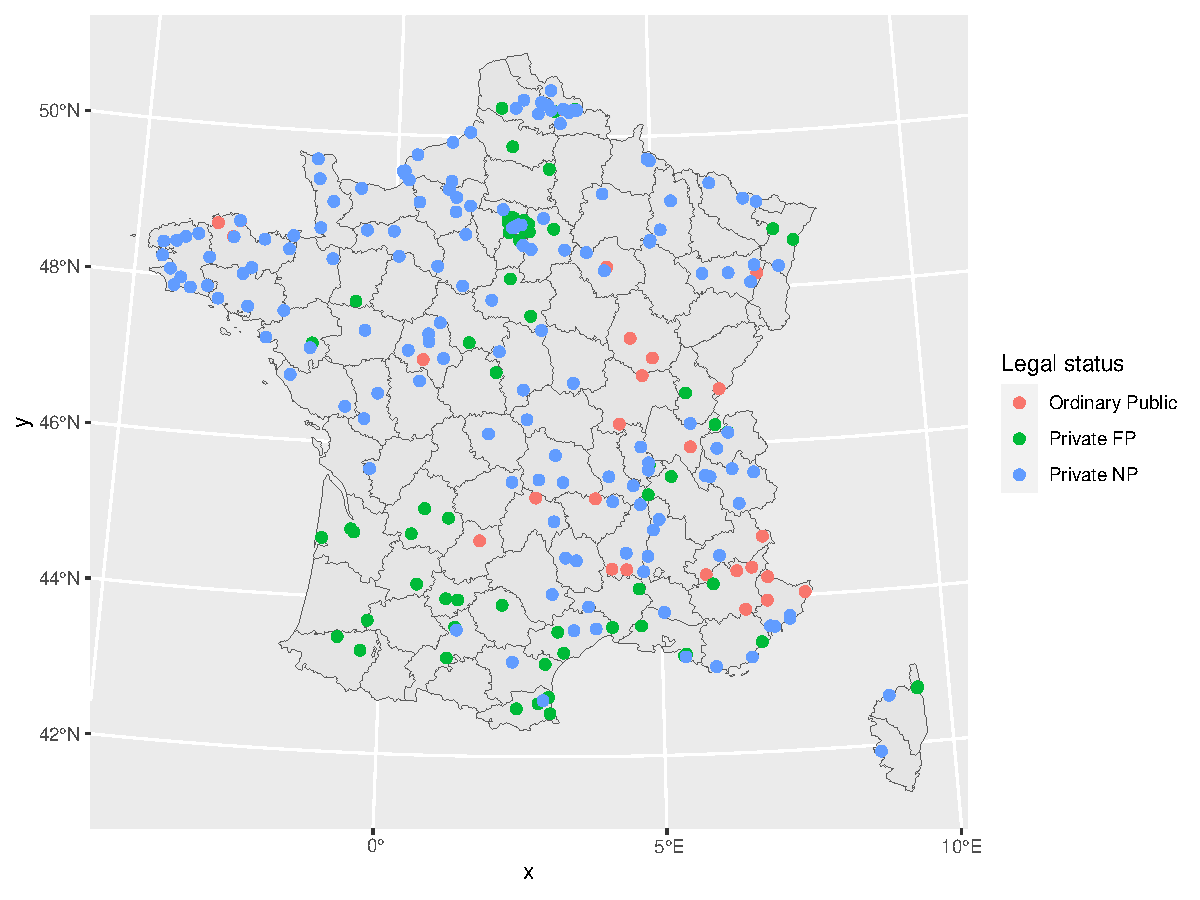
\includegraphics[width=0.9\textwidth]{../../Figures/2013-2022/Maps/Map.pdf}
  \end{figure}
\end{frame}

\begin{frame}[allowframebreaks]
  \frametitle{References}
  \bibliography{../Thesis/ref.bib}
  \bibliographystyle{apalike}
\end{frame}

\appendix

\begin{frame}[label=inputdemand]{Conditional Input Demand Function}
  In standard microeconomics, the profit maximization problem is
  \begin{equation*}
    \max_{\vec{y}} \sum k_i y_i - \sum p_i x_i \quad \text{subject to} \quad f_i(x_1, x_2, \ldots, x_n) = y_i
  \end{equation*}
  where $p_i$ is the price of input $i$ and $f$ is the cost function.

  The cost minimization problem is thus
  \begin{equation*}
    \min_{\vec{x}} \sum p_i x_i \quad \text{subject to} \quad f_i(x_1, x_2, \ldots, x_n) = y_i
  \end{equation*}
  Thus, the factor demand function/correspondence is
  \begin{equation*}
    x_i = x_i(p_1, p_2, \ldots, p_n, y_1, y_2, \ldots, y_m)
  \end{equation*}
  \hyperlink{literature}{\beamergotobutton{Back}}
\end{frame}

\begin{frame}[label=production]{Input demand function vs Production function}
  \begin{itemize}
    \item We can remain agnostic as to the nature of the appropriate formula for the
          aggregation of outputs and use as many different products as desired.
    \item When input prices have low variability. Conditional factor demand can be
          estimated without information on input prices. Even if we add prices, due a
          lack of variability, the price parameters will be poorly estimated.

    \item From $x_i = x_i(p_1, p_2, \ldots, p_n, y_1, y_2, \ldots, y_m)$, we do not need
          to observe a complete list of inputs. But we do need to observe all input
          prices (can be ignored if almost no variability) and all outputs. While in the
          production function, it is the other way around (need to observe all inputs).
          Since, in our case, output is more \textit{observable} than input (because
          capital is not easily observed), this approach is preferred.
  \end{itemize}
\end{frame}

\begin{frame}
  \frametitle{First glance}
  \begin{columns}[T,T]
    \column{0.5\textwidth}
    \makebox[\textwidth][c]{
      \fontsize{5pt}{5pt} \selectfont
      \input{../../Tables/2013-2022/reg_pool_iv_ex.tex}}

    \column{0.5\textwidth}
    \makebox[\textwidth][c]{
      \fontsize{5pt}{5pt} \selectfont
      \input{../../Tables/2013-2022/reg_dummy_iv_ex.tex}}

  \end{columns}
\end{frame}

\begin{frame}[label=reg_sep]{Second glance}
  \begin{table}
    \fontsize{6pt}{6pt}\selectfont
    \input{../../Tables/2013-2022/reg_sep_iv.tex}
  \end{table}
  \hyperlink{output}{\beamergotobutton{Back}}
\end{frame}

\begin{frame}
  \frametitle{Panel data Estimator}
  \begin{itemize}\itemsep=12pt
    \item Strict exogeneity: Within Group/First Diffrence
          \begin{equation*}
            E[\epsilon_{it}|x_{i1},\ldots, x_{iT},\theta_i]=0
          \end{equation*}
    \item Relaxed: First Difference GMM \citep{arellano1991some}, System GMM
          \citep{arellano1995another,blundell1998initial}.
          \begin{equation*}
            E[\epsilon_{it}|x_{i1},\ldots, x_{it-p},\theta_i]=0
          \end{equation*}
  \end{itemize}

  Issues: Weak instruments \citep{blundell_bond_1998} and the proliferation of
  instruments \citep{roodman2007short}.
  \begin{equation*}
    \E[\Delta x_{i,t-1}(y_{it}-\beta x_{it})] \quad \text{if}\quad \E\bra{\Delta x_{i,t-1}(\theta_i+\varepsilon_{i,t})}=0
  \end{equation*}
\end{frame}

\begin{frame}
  \frametitle{NPMLE Computation Methods}

  The primal problem:
  \begin{equation*}
    \min_{f=dG}\set{-\sum_i \log g(y_i)\bigg |g(y_i) = T(f),\ K(f)=1,\ \forall i }
  \end{equation*}
  where $ T(f)=\int p(y_i |\theta)fd\theta $ and  $K(f)= \int f d\theta$.\\
  Discretize the support:
  \begin{equation*}
    \min_{f=dG}\left\{-\sum_i \log g(y_i)\bigg |g=Af,\ {1^T}f=1\right\}
  \end{equation*}
  where $A_{ij}= p(y_i|\theta_j) $ and $ f = (f(\theta_1),f(\theta_2),\ldots,f(\theta_m))$.\\
  The dual problem:
  \begin{equation*}
    \max_{\lambda,\mu} \left\{ \sum_i \log \lambda_1(i) \bigg| A^T\lambda_1 < \lambda_2 1,\ (\lambda_1>0) \right\}
  \end{equation*}
\end{frame}

\begin{frame}[label=normality]{Normality assumption on $\varepsilon_{it}$}
  Estimate the fixed effect $\theta_i$ by
  \begin{align*}
    \hat{\theta}_i =                       & \frac{1}{T}\sum(\theta_i+\varepsilon_{it}+x_{it}(\beta-\hat{\beta})) \\
    \overset{N\to \infty}{\longrightarrow} & \theta_i+\frac{1}{T}\sum_t \varepsilon_{it}
  \end{align*}
  When $T$ is relatively small (or even fixed), can't use central limit theorem to claim that $\hat{\theta}_i \overset{d}{\to} \caln(\theta_i,\frac{\sigma_i^2}{T})$.
  $\longrightarrow$ Assume that $\varepsilon_{it} \sim \caln(0,\sigma_i^2)$ .
  \hyperlink{observation}{\beamergotobutton{Back (main)}}   \hyperlink{limitation}{\beamergotobutton{Back (end)}}
\end{frame}

\begin{frame}
  \frametitle{$G(\theta,\sigma)$: Posterior Mean}
  \begin{figure}
    \centering
    \includegraphics[width=0.9\textwidth]{../../Figures/2013-2022/GMM_fd/GLVmix/Left_0.2_0.2_PMKWs.pdf}
  \end{figure}
\end{frame}

\begin{frame}
  \frametitle{$G(\theta,\sigma)$: James-Stein Shrinkage}
  \begin{figure}
    \centering
    \includegraphics[width=0.9\textwidth]{../../Figures/2013-2022/GMM_fd/GLVmix/Left_0.2_0.2_JS.pdf}
  \end{figure}
\end{frame}

\begin{frame}[label=tpcontour]{TP vs PM}
  \begin{figure}
    \centering
    \includegraphics[width=0.9\textwidth]{../../Figures/2013-2022/GMM_fd/GLmix/Contour_Left_0.2_0.1_TPKWs_PMKWs.pdf}
  \end{figure}
  \hyperlink{tpselect}{\beamergotobutton{Back}}
\end{frame}

\begin{frame}{TP vs JS}
  \begin{figure}
    \centering
    \includegraphics[width=0.9\textwidth]{../../Figures/2013-2022/GMM_fd/GLmix/Contour_Left_0.2_0.1_TPKWs_JS.pdf}
  \end{figure}
\end{frame}

\begin{frame}{TP vs MLE}
  \begin{figure}
    \centering
    \includegraphics[width=0.9\textwidth]{../../Figures/2013-2022/GMM_fd/GLmix/Contour_Left_0.2_0.1_TPKWs_MLE.pdf}
  \end{figure}
\end{frame}

\end{document}
